This component models the out-going interface through which packets representing either commands (in a service user application) or reports (in a service provider application) are sent to their destination. The OutStream is therefore located at the interface between an application and the middleware layer. 

An application A may send packets to several destinations. The packets may either originate within application A itself or they may have originated in some other application (the latter is the case if application A is re-routing the packets). Depending on the characteristics of the middleware, only one OutStream component may be present in application A with the multiplexing of the out-going connections to the packet destinations being done in the middleware, or several OutStream components may be present each handling packets to a subset of destinations. If an application is sending internally generated packets to a certain destination D and is also re-routing packets to the same destination D, then it must use the same OutStream for both kinds of packets. 

The OutStreams are responsible for assigning the sequence counter attributes of out-going packets generated by an application. Since sequence counters are incremented according to a packet's group, all packets belonging to the same group must go through the same OutStream.

The OutStream component extends the Base Component of section \ref{sec:BaseCmp} and it therefore inherits the initialization and configuration logic defined by the Base Component. In the initialization and configuration process, the OutStream is linked to the middleware. This process is necessarily application-specific (because the middleware is not specified by the CORDET Framework). However, the CORDET Framework specifies that an OutStream component may only become configured (i.e. it may enter state CONFIGURED) after the middleware connection has become available (it has entered state AVAIL). This ensures that an OutStream only becomes configured after its middleware connection has terminated its own initialization and configuration process.

\begin{figure}[ht]
 \centering
 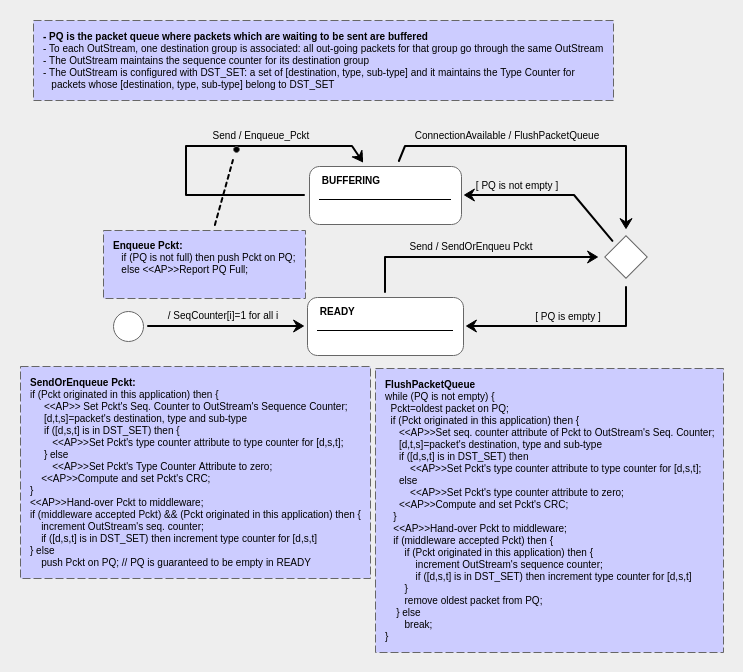
\includegraphics[scale=0.42,keepaspectratio=true]{OutStream.png}
 \caption{The OutStream State Machine}
 \label{fig:OutStream}
\end{figure}

In state CONFIGURED, the behaviour of an OutStream is described by the state machine of figure \ref{fig:OutStream} (the \textit{OutStream State Machine}). The state machine has two states: READY and BUFFERING. State READY represents a situation where the connection is expected to be available and the OutStream hands over packets to the middleware. State BUFFERING represents a situation where the connection may be unavailable and where packets are buffered without being handed over to the middleware.

The OutStream State Machine reacts to two commands: \texttt{Send} and \texttt{ConnectionAvailable}. Command \texttt{Send} is issued by the host application when it wishes to send a packet to its destination. If, at the time a \texttt{Send} request is made, the state machine is in state BUFFERING, then the packet is enqueued in the \textit{Packet Queue}. 

The Packet Queue is an internal data structure where packets which are waiting to be sent are stored. The size of the packet queue is fixed and is defined as part of the OutStream configuration. Attempts to enqueue a packet in a full queue are reported as errors.

The Packet Queue is a FIFO queue. This guarantees that the OutStream component delivers packets to the middleware in the same order in which it receives them from its host application. 

If, instead, a \texttt{Send} request is made at a time when the OutStream is in state READY, then an attempt is made to hand over the packet to the middleware. If this succeeds, the OutStream remains in state READY. If instead the hand-over to the middleware fails, the packet is enqueued and the OutStream makes a transition to state BUFFERING. Note that the logic of the OutStream State Machine guarantees that, at entry into state READY, the packet queue is empty.
 
The \texttt{Send} command may either fail or succeed. If it results in its packet being enqueued on the Packet Queue, then the \texttt{Send} command succeeds (note that property P3 below ensures that a packet which has been enqueued will eventually be handed over to the middleware). If instead it results in its packet being lost because, at the time the \texttt{Send} command was called, the Packet Queue was full, then the \texttt{Send} command fails. 

Command \texttt{ConnectionAvailable} would typically be generated by the middleware when the connection (or one of the connections) associated to the OutStream changes from NOT\_AVAIL to AVAIL. This command is used to trigger the flushing of the Packet Queue. When the OutStream receives command \texttt{ConnectionAvailable} it empties the Packet Queue one packet at a time until the queue is empty or the connection becomes unavailable.

The out-going packets which are handled by an OutStream may have two origins: (a) they may have originated in the same application to which the OutStream belongs, or (b) they may be re-routed packets which originate from some other application and which are using the OutStream's application as a gateway on the way to their destination (see figure \ref{fig:PcktInterfaceConcept}). In case (a), the OutStream is responsible for setting the sequence counter and type counter attributes of the out-going packet. In case (b), by contrast, the packet's sequence counter and type counter attributes are already set (they have been set by the application where the packet originated).

In case (a), the mamagement of the sequence counter is based on the fact that the sequence counter counts the number of packets sent to a destination group and that there is an OutStream for each destination group. Hence, each OutStream maintains one sequence counter which it increments every time it successfully hands over a packet to the middleware.

The management of the type counter is instead more complex. The Type Counter is an optional attribute whose value represents the number of packets sent to a given triplet of [destination, type, sub-type]. An OutStream is therefore configured with a set called DST\_SET reprensenting all the [destination, type, sub-type] triplets for which a Type Counter is maintained. For each entry in this set, the OutStream maintains a Type Counter which it increments when a packet of the corresponding destination, type and sub-type is successfully handed over to the middleware. Packets whose [destination, type, sub-type] are not in DST\_SET have their Type Counter set to zero.

The OutStream is responsible for computing and setting the CRC of an out-going packet. This can only be done after the sequence counter and type counter have been set (because the value of two counters contributes to the value of the CRC).
 
